% Author: Joshua Carey

%
\let\textcircled=\pgftextcircled\chapter{Methodology}

% graph TD
%     Start -->Tools[Decide Tools]
%     Tools --> |Enviroment| Environment{Unity}
%     Tools --> |RL| MLAgents{MLAgents}
%     Environment -->|Create simulation| Models{Models}
%     Models --> collisionDetection[Collision Detection]
%     Models --> boatModel[Boat Model]
%     Models --> kiteModel[Kite Model]
%     boatModel --> Agent
%     kiteModel --> Agent
%     MLAgents --> Agent
%     Agent --> Actions
%     Agent --> Observations
%     Agent --> Rewards
%     Actions --> Training(Training)
%     Observations --> Training
%     Rewards --> Training
%     Training -->|Curriculum| optimisation
%     optimisation -->AdjustParameters[HyperParameters]
%     AdjustParameters --> Training
%     AdjustParameters --> Output
% \initial{T}he following chapter will discuss the steps taken to create a robust reinforcement learning solution that is capable of controlling a kiteboat. It will start by explaining the tooling used to create the RL algorithm and the environment, before moving on to the implementation of the environment and the Agent. Finally it will discuss the training process and optimisation. The development process discussed in this chapter can be seen in figure$~$\ref{development_process}.

\initial{T}his chapter outlines the methodology used to develop an autonomous control system for a kite-powered vessel using Reinforcement Learning (RL). It begins with an overview of the essential tools, including the MLAgents toolkit and its integration with Python and PyTorch, crucial for the RL algorithm and the simulation environment. The focus then shifts to the development of the simulation environment, detailing the boat and kite models and the assumptions underlying their design.

% Key to the simulation is the implementation of the Gilbert-Johnson-Keerthi (GJK) algorithm for collision detection and the establishment of control mechanisms for both autonomous and manual operation. 

The chapter delves into the RL implementation, discussing the agent script and the dynamics of observations, actions, and rewards that guide the agent's learning within the Unity environment. Finally, the chapter covers the training process, highlighting the use of Curriculum Learning to enhance the agent's learning efficiency and the optimisation strategies employed, including hyperparameter tuning and the utilisation of the Blue Crystal High-Performance Computing (HPC) facility. This section aims to provide an understanding of the computational efforts and processes that were pivotal in the project’s development, shown in figure$~$\ref{development_process}. All environment scripts discussed in the methodology can be found in the \texttt{ai\_kite/Assets/Scripts} directory of the project files.

\begin{figure}[h]
    \centering
    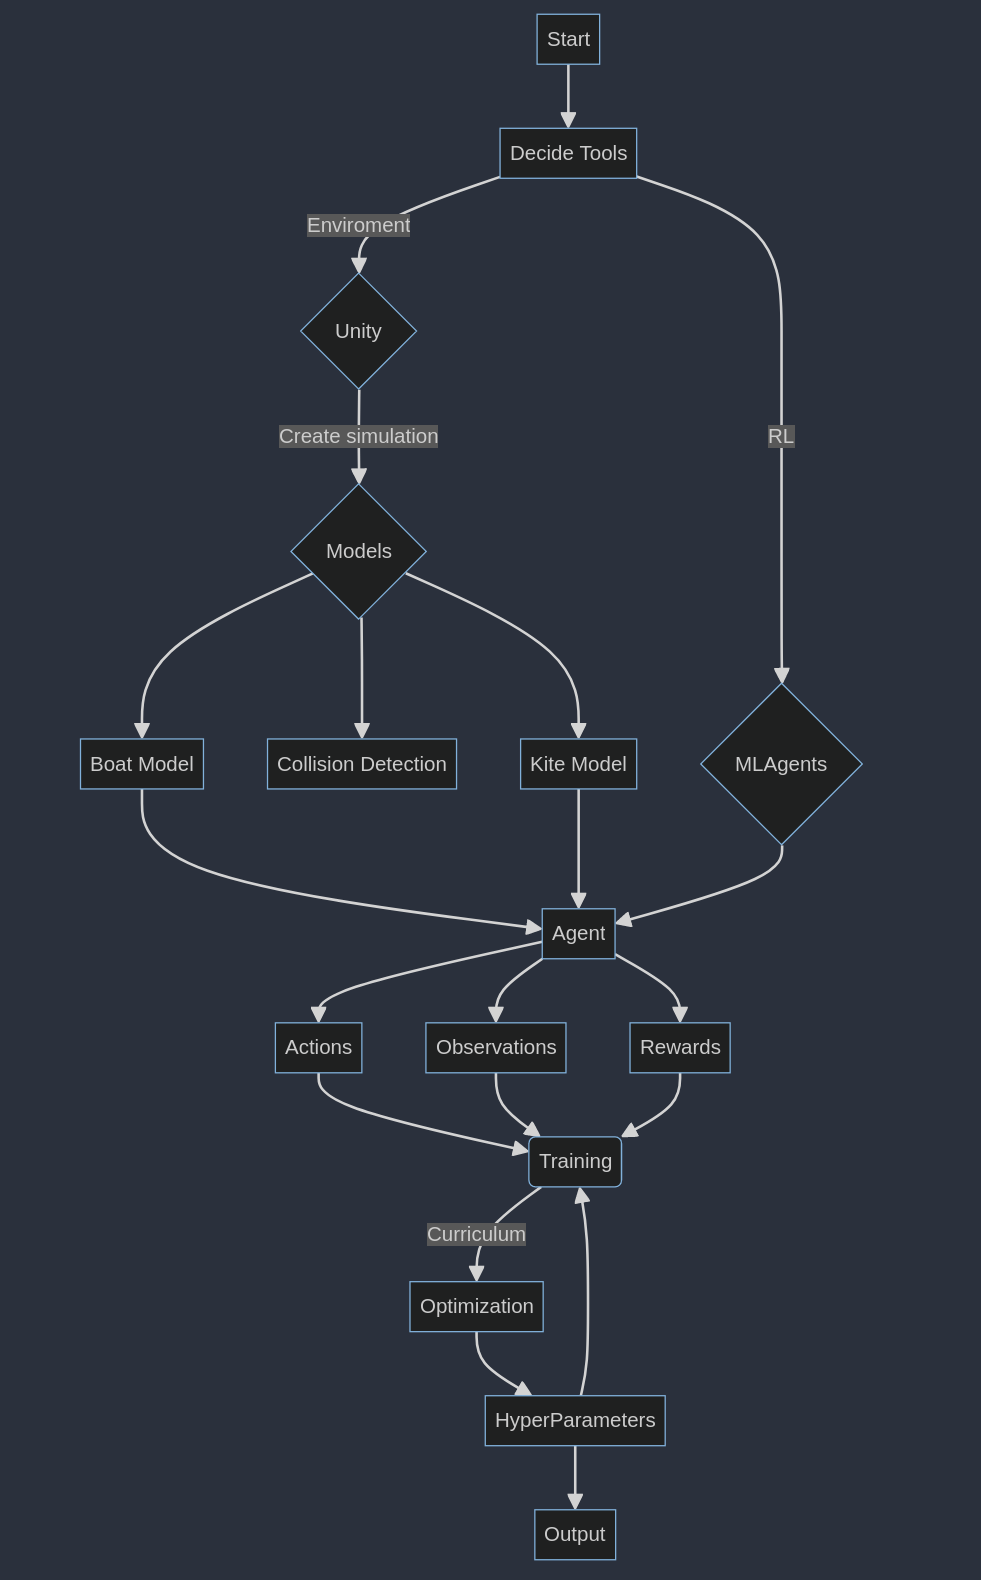
\includegraphics[width=0.5\textwidth]{Images/method.png}
    \caption{Development Process}\label{development_process}
\end{figure}

\section{MLAgents}
MLAgents is an open-source project that allows games and simulations to serve as the environment for training intelligent agents. At its core MLAgents utilises RL, although it also supports other methods such as imitation learning.

\subsection{Python Implementation}
% The neural network used in the reinforcement learning is implemented in Python.

MLAgents toolkit is a Python Library that acts as an interface between the environment (gym), in this case Unity, and PyTorch$~$\cite{paszke2019pytorch}. PyTorch is an open-source machine learning library based on the Torch library, known for its flexibility, ease of use, and native support for GPU acceleration, which is essential for the computation-heavy processes involved in training neural networks. Torch is a Python-based scientific computing package that provides prebuilt components for machine learning and deep learning, as well as a wide range of mathematical functions. MLAgents uses a low level API to communicate directly with the Unity environment (\texttt{mlagents\_envs}) frame by frame, and an entry point to train (\texttt{mlagents-learn}). This stepping process allows for the synchronous collection of observations, executions of actions and retrieval of rewards. 


The algorithm used in this project is a Proximal Policy optimisation (PPO) network, and so will utilise the actor-critic method as discussed in section$~$\ref{sec:ppo_background}.

RL, preveously discussed in section$~$\ref{RL_background}, is an approach to learning where an agent learns to make decisions by interacting with its environment. The fundamental components of this interaction with the environment are observations, actions and rewards.
\begin{itemize}
    \item Observations (State): These are the pieces of information that the agent receives from the environment at each step or frame. In Unity, observations are collected through sensors or manually coded to be extracted from the game objects. They are typically fed into the neural network as a vector of floating-point numbers, representing the current state of the environment.
    \item Actions: Based on the observations, the agent takes actions which are the outputs of the neural network. These actions can be discrete (e.g., turn left, turn right) or continuous (e.g., change angle by a certain degree). The neural network's output layer is designed accordingly to provide the appropriate action space for the agent. (Configured as part of the behavioural parameters in Unity)
    \item Rewards: After taking an action, the agent receives a reward signal, which is a numerical value indicating how well the action contributed to achieving its goal. This reward is used to adjust the neural network's weights, with the aim of maximising the total accumulated reward.
\end{itemize}
A full breakdown of the actions, observations, rewards, and how the agent script configures these for this project can be found in section$~$\ref{sec:RL_Implementation}.

A sequence diagram of the interaction between the Unity environment and the Python neural networks, can be seen in figure$~$\ref{MLAgents_Seq_Diagram}.

\begin{figure}[h]
    \centering
    \resizebox{\textwidth}{!}{%
    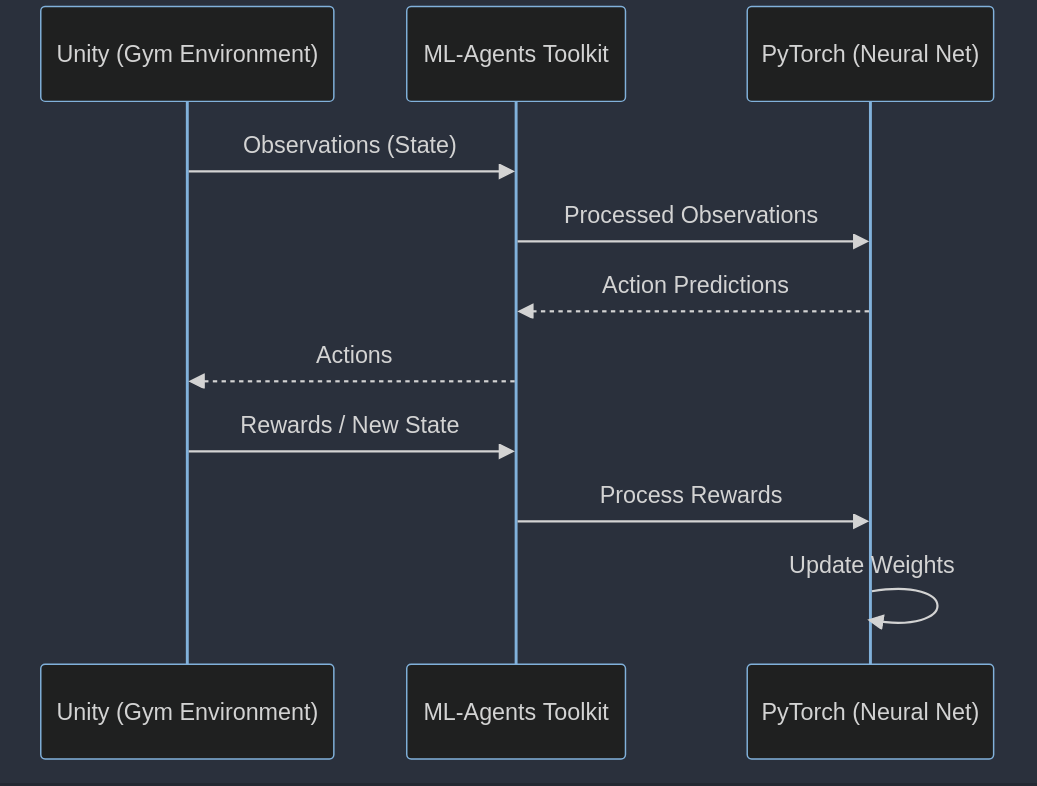
\includegraphics[width=0.5\textwidth]{Images/MLAgents_Seq_Diagram.png}
    }
    \caption{MLAgents Sequence Diagram}\label{MLAgents_Seq_Diagram}
\end{figure}

% sequenceDiagram
%     participant Unity as Unity (Gym Environment)
%     participant MLAgents as ML-Agents Toolkit
%     participant PyTorch as PyTorch (Neural Net)

%     Unity->>MLAgents: Observations (State)
%     MLAgents->>PyTorch: Processed Observations
%     PyTorch-->>MLAgents: Action Predictions
%     MLAgents-->>Unity: Actions
%     Unity->>MLAgents: Rewards / New State
%     MLAgents->>PyTorch: Process Rewards
%     PyTorch->>PyTorch: Update Weights


% \begin{figure}[h]
%     \centering
%     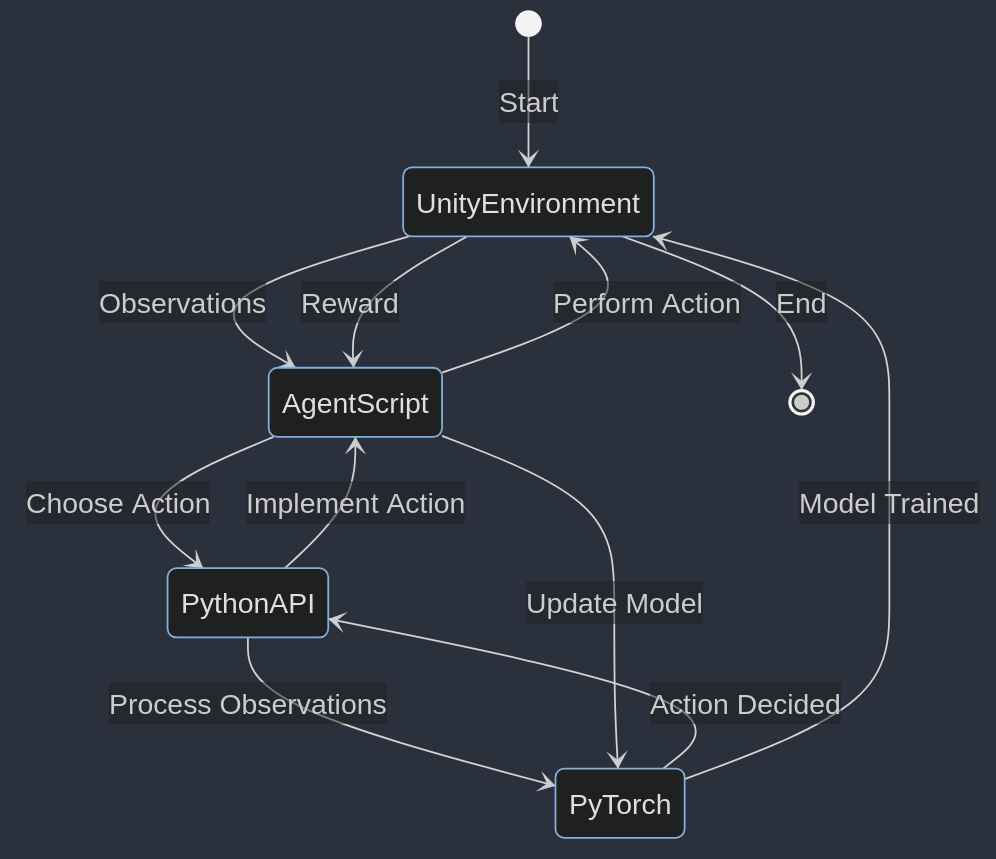
\includegraphics[width=0.5\textwidth]{Images/unity_mlagents.png}
%     \caption{MLAgents Integration}\label{MLAgents_Integration}
% \end{figure}



The technical instructions to setup MLAgents in Python and Unity are as follows:
% \newline$~$\url{https://github.com/lipj01/AI-Kite-Control} CHANGE TO MY REPO
\begin{itemize}
    \item Initialise a python virtual environment
    \item Install MLAgents with the command: \texttt{pip install mlagents}
    \item Configure Unity project to use MLAgents by importing the MLAgents package, see section$~$\ref{sec:RL_Implementation} for more details.
\end{itemize}

\section{The Environment}\label{sec:env}

The first step to this process is to create the environment, which the agent will use to train. In this case that will need to look something like a sailing game; it will have some form of water, a boat, a kite and a course. 
% For any machine learning endeavor, especially one with such intricate physical dynamics, the choice of simulation environment is paramount. Not only does it provide the playground for our AI agent to learn and make mistakes safely, but it also serves as a litmus test for the robustness and realism of the designed model.

% Given the myriad of choices available, the Unity game engine emerged as the most suitable platform. Its native support for machine learning applications through the MLAgents toolkit was unmatched. Beyond its reputation in gaming, the inherent support for mesh bodies, colliders, and a variety of joints made it an attractive option for simulating the kite-boat system, which comprised a complex dance of forces, and counterforces. Unity is recognized for its potent physics engine, however for this project the use of Unity's physics engine will be kept to a minimum, with an emphasis on implementing as much of the simulation from scratch as possible. Unity will be used primarily for its visual capabilities and the ability to be used as the gym environment for machine learning simulations. 

% Central to our simulation is the depiction of water, the medium in which our boat will navigate. Here, the Unity HDRP Water System 16.0.3$~$\cite{UnityHDRPWaterSystem} came to the rescue. Bundled with Unity 2023.2.0b9, this water system provides a realistic representation of water with its undulating waves, refractions, and reflections. 
% The alternative option to using Unity's water system was to model an entire particle fluid simulation, this would have had its advantages, however it would have been a lot more computationally expensive and would have taken a lot longer to implement. As this project was primarily focused on training a RL algorithm for controlling a kiteboat it was decided that the Unity water system would be sufficient for this project.  

The boat part of the kiteboat had two main component scripts, the buoyancy and the rudder, allowing the boat to float and be steered. The implementation of Buoyancy and the rudder are discussed in more detail in section$~$\ref{sec:Boat}. The kite had a single script that defined the physics and its explanation can be found in section$~$\ref{sec:Kite}. The final training environment can be seen in figure$~$\ref{training_enviroment}. 

% full width image
\begin{figure}[h]
    \centering
    \resizebox{\textwidth}{!}{%
    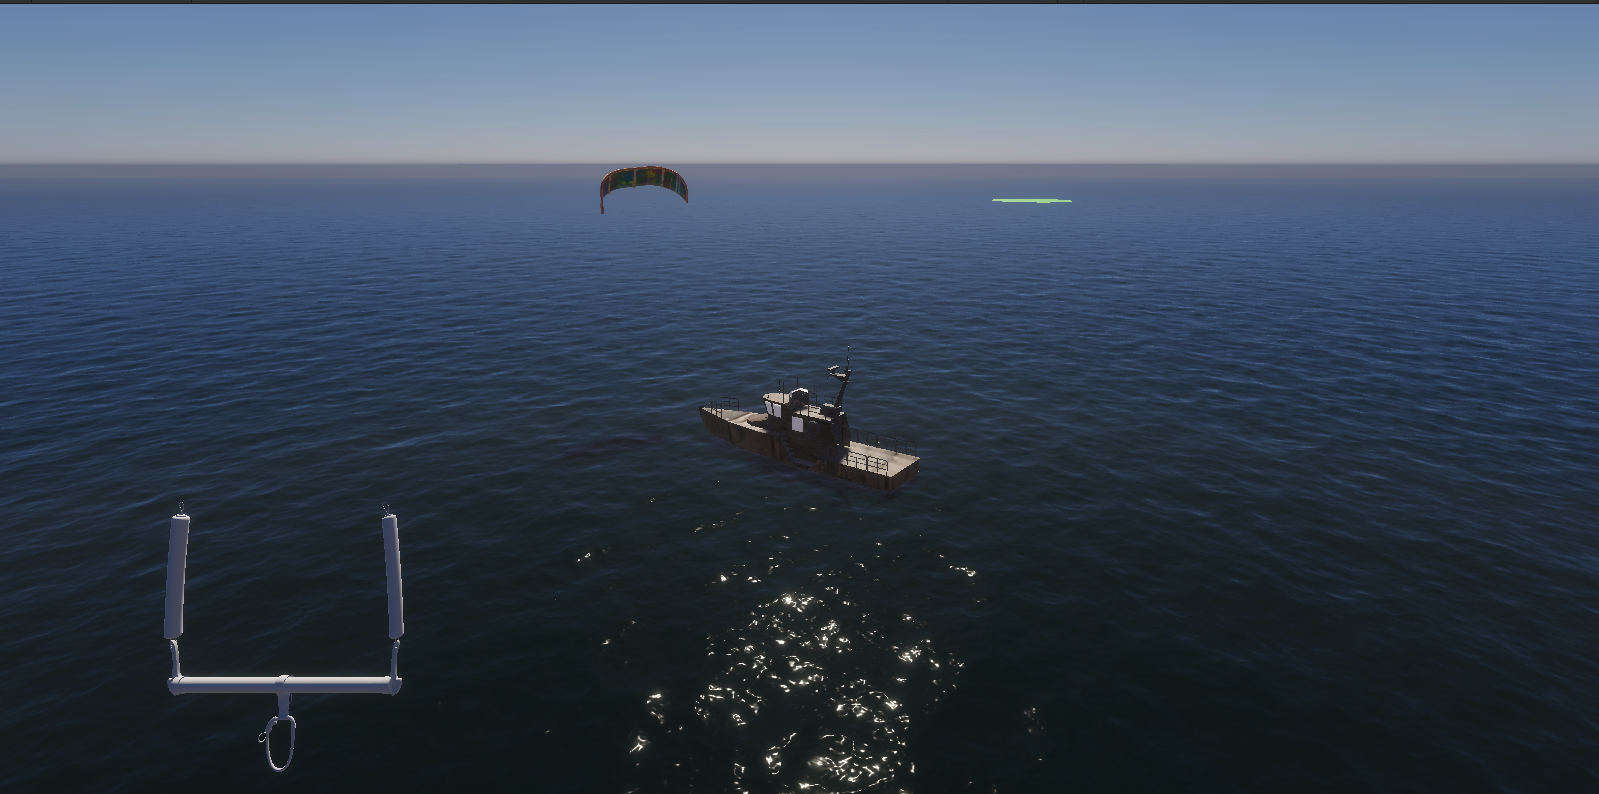
\includegraphics[width=0.5\textwidth]{Images/TrainingEnv.png}
    }
    \caption{Training Environment}\label{training_enviroment}
\end{figure}


\subsection{Boat Model}\label{sec:Boat}

As with any simulation the first step was to define a series of assumptions that would simplify model.

\textbf{Boat Assumptions}
\begin{itemize}
    \item The Archimedes force is uniform across all submerged sections of the boat.
    \item The rudder forces of lift and drag could be aproximated to a torque applied about the rear of the boat.
    \item Once the boat is moving at a speed greater than 0.25m/s the lift and drag forces of the keel are equal to the downwind component of the kite's resultant force- essentially providing a non'slip condition.
\end{itemize}
Buoyancy, the force that allows ships to float, was the first physical property to be addressed. Rooted in Archimedes' Principle, it dictates that the buoyant force exerted on a submerged body is equivalent to the weight of the fluid displaced by that body. In our Unity environment, the boat's hull, represented as a `mesh', was divided into many small triangles or Voxels. These Voxels became the fundamental units for calculating buoyancy, allowing for a granular and realistic representation of the boat's interaction with water. This was achieved by first calculating the total Archimedes force (AF) of the entire boat using equation$~$\ref{archimedes}, followed by a local AF at each Voxel. The water level, y component, was then computed at each voxel's (x,z) coordinates to determine if it was above or below the surface. If below the surface the component of the AF was applied vertically at each voxel.

\begin{equation}
    F_B = \rho_{w}gV
    \label{archimedes}
\end{equation}

While buoyancy ensures our boat doesn't sink, it's the rudder that grants it direction. The Rudder.cs script handles the implementation of the rudder and the keel. The equation for the torque applied about the rear of the boat is shown in equation$~$\ref{rudder_torque}. 

% the torque equation
% float turnForce = angle * boatForwardSpeed * rotationScale;
% boatRb.AddTorque(transform.up * turnForce);
\begin{equation}
    \tau = \alpha v R
    \label{rudder_torque}
\end{equation}

where $\tau$ is the torque, $\alpha$ is the angle of the rudder, $v$ is the speed of the boat and $R$ is the rotation scale.

\subsection{Kite Model}\label{sec:Kite}
Capturing the intricate movements of a kite as it fly's through the air involves a complex balance between theoretical aerodynamics and the unpredictability of real-world conditions. In this model several assumptions were made to streamline the complexity into a more manageable form and are shown below.

\textbf{Kite Assumptions}
\begin{itemize}
    \item The kite is modelled as a symmetrical aerofoil, with constant lift and drag coefficients.
    \item Constant wind angle and laminar flow over the entire kite.
    \item The kite is always in the air, for the initial model the case where the kite crashes and requires relaunching was not considered. This would require adding buoyancy to the kite.
\end{itemize}

This sections outlines a kite model that, while simplified, serves as an effective tool for designing and testing the RL algorithm. The model is geared towards a realistic representation of the kites behaviour and its response to control inputs. The kite chosen for this project was a Leading Edge Inflatable (LEI) kite, which is the most popular and mass produced recreational style of kites that exists. These kites connect to a control bar via 4 dyneema kite lines. Two center power lines take the load of the kite, while the outside two are responsible for steering, as shown in figure$~$\ref{kite_diagram}.

% insert kite diagram
\begin{figure}[h]
    \centering
    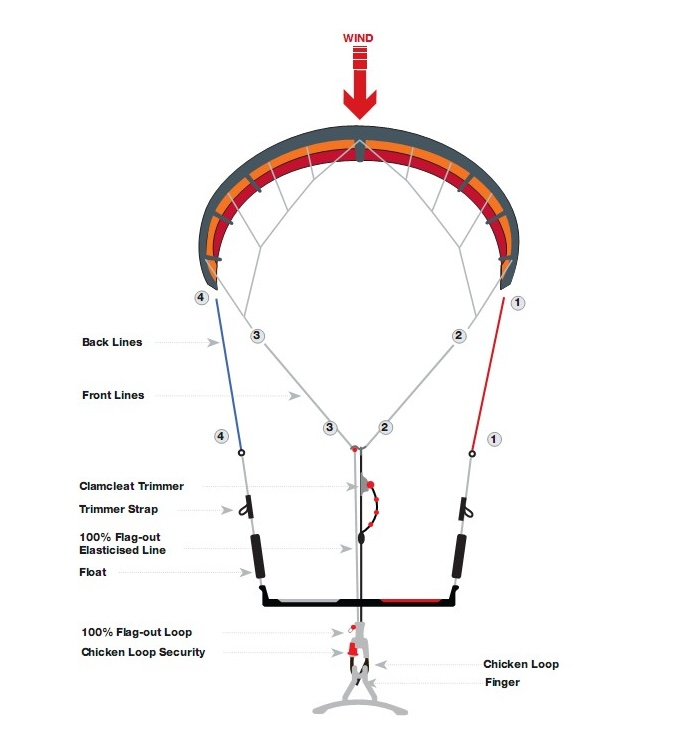
\includegraphics[width=0.5\textwidth]{Images/kitediagram.jpg}
    \caption{LEI Kite Diagram}\label{kite_diagram}
\end{figure}

The kite model was implemented using the kite.cs script. The kite was modelled as a symmetrical aerofoil, and implemented as a rigid body with constant lift and drag coefficients. The lift and drag forces were calculated using the equations shown in equation$~$\ref{lift} and equation$~$\ref{drag}.
\begin{equation}
    F_L = \rho C_L A \frac{v^2}{2} 
    \label{lift}
\end{equation}
\begin{equation}
    F_D = \rho v^2 C_D A \frac{v^2}{2} 
    \label{drag}
\end{equation}

where $F_L$ is the lift force, $F_D$ is the drag force, $\rho$ is the density of air, $C_L$ is the lift coefficient, $C_D$ is the drag coefficient, $A$ is the area of the kite and $v$ is the velocity of the kite relative to the wind.

In order to replicate the kite's mechanics and bar configuration, the model uses 4 configurable joints. These joints were fixed at certain lengths from the deck of the boat, designed to permit movement across all rotational axis without any `bounce' effect. This design enables the kite to descend or `fall' in conditions of low wind, mirroring real-world behaviour where the kite may lose altitude but can be menoeuvered back into position. To simulate the bar being pulled in, the lift and drag coefficients were increased, this has the effect of increasing the angle of attack of the kite.


\subsection{Collision Detection}
The Gilbert-Johnson-Keerthi (GJK)$~$\cite{gilbert88gjk} algorithm is a sophisticated method for collision detection between convex shapes. This algorithm was the approach taken to detect weather the kiteboat had reached the waypoint during training, and later, to work out if it had rounded the marks of the racecourse. 
% The implementation of the GJK algorithm can be found in the GJK.cs script of the unity project or section$~$\ref{sec:gjk} of the appendices.
The GJK algorithm operates by iterative refinement of a simplex, which is a set of points that can define a line segment, triangle, or tetrahedron. The algorithm progresses by assessing whether the simplex contains the origin, which would imply an overlap between the two shapes. The initial direction d is determined by the normalised vector from center of object 1 to the center of object 2, constrained in the x-z plane by nullifying the y component, meaning the algorithm is only concerned with the horizontal plane.  

Within the GJK method, the Support function plays a pivotal role, calculating the Minkowski difference between the two shapes in a specified direction. This is achieved by finding the farthest points along that direction on both shapes and then subtracting them to obtain a single point in the Minkowski space.

The HandleSimplex function is a recursive strategy that adjusts the simplex and direction d based on whether the current simplex is a line or triangle. For a line, the LineCase function is invoked, and for a triangle, the TriangleCase is employed. These functions adjust the simplex and direction of search to move closer to the origin, if it is not already contained within the simplex.

% \subsection{Mark Roundings}

\section{Controls}
In order to ensure the agent would be able to learn to sail the kiteboat a playable game version was created. As discussed above the kite was modelled using 4 configurable joints to replicate the line system. There are several ways of configuring these so that a simple control input will result in the desired movement of the kite. The controls chosen for this project were 6 discrete actions, shown in table$~$\ref{actions}, allowing the kiteboat to be steered and the kite to be flown. 


\section{RL Implementation}\label{sec:RL_Implementation}

In order to use Unity game engine as the environment for RL it must be setup correctly, the steps are as follows:
\begin{enumerate}
    \item Enable MLAgents in Unity:
    Window $\rightarrow$ Package Manager $\rightarrow$ MLAgents $\rightarrow$ Install
    \item Create an empty game object in the scene.
    \item Create a new \texttt{C\#} script of with class of type `agent' and attach it to the game object, include the methods discussed in subsection$~$\ref{agent_script}.
    \item Add the Behaviour Parameters component to the game object.
    \item Create a new agent config file (\texttt{.yaml}) and set the `Behavioural Name' in the Behaviour Parameters component to the name of the config file.
\end{enumerate}  
% A visual representation can be found in section$~$\ref{sec:unity_setup} of the appendix.

\subsection{The Agent Script}\label{agent_script}
The kiteboat agent sets up the scene for learning and in order for Unity to correctly process the script it must have the following 4 functions implemented:
\begin{itemize}
    \item OnEpisodeBegin()
    \item CollectObservations(VectorSensor sensor)
    \item OnActionReceived(ActionBuffers actions)
    \item Heuristic(in ActionBuffers actionsOut)
\end{itemize}

These are the minimum requirements for the agent setup, however there are several other functions that can be implemented to further customise the agent, handle errors and provide additional information. The agent starts by taking in the Kite and the Boat rigid bodies, as well as the rudder and kite scripts. A new gjkCollisionDetection is also initialised. The script starts with the OnEpisodeBegin method, which in turn starts by ensuring the training environment has been reset. The reset method sets the velocities and angular velocities of all rigid bodies in the scene to 0 and returns the kiteboat to a starting position. The remaining methods will be discussed in more detail below.


\subsection{Observations}
CollectObservations provides the network will all the information about the State of the environment, and so aims to provide all the required information for the agent to make an informed decision. This means fully describing the movement of the kite and boat, as well as the position of the boat relative to the waypoint, allowing it to gain an idea of direction. It is easy to see how the number of observations could rapidly increase, but this would also increase the complexity of the network and the likelihood of the agent becoming `confused' by the data its receiving. With this in mind the goal is to provide all the required information about the state in the minimum number of observations possible, this is achieved by combining vectors where appropriate. Another consideration when thinking about the observations was that they should be possible to collect if this system were to be created in the real world. This means that the observations should be possible to collect using sensors, such as GPS, wind speed and direction, and accelerometers. The observations used in this project are shown in table$~$\ref{observations}.

\begin{table}[h]
    \centering
    \begin{tabular}{c|c|c}
        Observation & Vector Size & Description \\
        \midrule
        Distance to the waypoint & 1 & The distance to the waypoint from the boat \\
        Boat Speed & 1 & The speed of the boat in the forwards direction \\
        Wind vector & 3 & The direction of the wind \\
        Relative Boat Angle & 1 & The angle of the boat relative to the wind \\
        Kite Position & 3 & polar angles of the kite relative to the wind\\
        Relative velocity of the kite & 3 & The velocity of the kite relative to the boat \\
        Kite altitude & 1 & The height of the kite above sea level \\
        Rudder Angle & 1 & The angle of the rudder \\

        \hline
    \end{tabular}
    \caption{Observations}\label{observations}
\end{table}

The total number of observations passed to the network is 14, this is a relatively small number of observations and so the network should be able to process them quickly. When providing observations to an agent is is essential they have no discontinuity in their values, as this can cause the network to become unstable. Observations that may be discontinuous are normalised to a value between 0 and 1. Normalised observations can increase the learning speed of algorithms, as the network does not have to learn the scale of the observations.

\subsection{Actions}
When the agent starts to train it has no idea what to do, it is essentially a blank slate, so starts by randomly flicking around the actions. The agent was given a discrete action space of 6 actions, these are shown in table$~$\ref{actions}. The actions are passed to the network as a vector of discrete 6 values (i.e float of either 0 or 1). The network then interprets these values and outputs the appropriate action. The actions are then passed to the OnActionReceived method, which in turn calls the methods that control the kite and boat. Discrete actions were chosen so that the rate of change of the angles that control the rudder and kite are not the choice of the network. Some brief experimentation with continuous actions showed the agent was prone to extremes. By limiting the rate of change of the rotations it gives the network an easier job and means the amount of freedom the network has can be configured. i.e. if the network could pick any value between 0 and 1 for the bar position, it would see far more aggressive controls making it harder for a stable flight to be achieved. On the other had the discrete action space encourages the agent to make a decision and stick with it while the action is being applied, this behaviour was further encouraged with the reward functions. 

These actions were tested as part of making a playable game, where the agent receives the same actions as a human controlling the kiteboat simulation. The Heuristic method that is one of the required functions for the agent script, allows the agent to be controlled by a human when no model is present. This is useful for testing the environment and the controls, as well as for playing the game. The Heuristic method takes in the action vector and sets the values of the actions to the values of the keyboard inputs. The keyboard inputs are set in the Unity editor and are shown in table$~$\ref{actions}. 

\begin{table}[h]
    \centering
    \resizebox{\textwidth}{!}{%
    \begin{tabular}{c|c|c|c}
        \textbf{Action} & \textbf{States} & \textbf{Description} & \textbf{Keyboard Input}\\
        \midrule
        Kite Bar Position & Left, Off, Right & Turns the bar to the right or left & Arrow left/right \\
        Rudder Angle & Left, Off, Right & The angle of the rudder & Keys `A' and `D'\\
        % Kite Bar Power & 0, 1 & The power of the kite bar & Space Bar \\
        \hline
    \end{tabular}
    }
    \caption{Actions}\label{actions}
\end{table}


\subsection{Rewards}

The rewards provided to the agent each step are the fundamental input that influences the future actions taken by the neural network, and so must be carefully applied when the agent performs positive actions and penalised when it performs negative actions. The reward function is the most important part of the RL algorithm, as it is the only way the agent can learn. The reward function is also the most difficult part of the RL algorithm to get right, as it is very easy to create a reward function that does not encourage the desired behaviour, moreover it is common to create a reward function that helps the agent fall into local maxima while training, especially with complex tasks. Table$~$\ref{rewards} shows the rewards used in this project, These rewards were however not all applied at the same time, they were applied in stages as the agent progressed through the curriculum. This is discussed in more detail in the following section$~$\ref{sec:training}.


\begin{table}[h]
    \centering
    \resizebox{\textwidth}{!}{%
    \begin{tabular}{c|c|c|c|c}
        \textbf{Reward} & \textbf{Condition} & \textbf{Value} & \textbf{Timing} & \textbf{Description/Impact} \\
        \hline
        \multirow{3}{*}{Boat Forward Speed} & >1m/s & +0.005 & Every Step & \multirow{3}{*}{Optimise the boat for forward speed} \\
                                               & >4m/s & +0.01  & Every Step &  \\
                                               & <0.1m/s & -0.001 & Every Step &  \\
        Rudder Angle & > 60$^{\circ}$ & -0.001 * abs(rudderAngle-60) & Every Step & Penalise the agent for aggressive steering \\
        \multirow{2}{*}{Distance to Waypoint} & current < previous\footnotemark[1]& +$\frac{10}{current}$ &Every Step & \multirow{2}{*}{Encourage the agent to move towards the waypoint}  \\
                                                  & current > previous & -0.01 * (current - previous) & Every Step &  \\
        Waypoint Reached & Waypoint Reached & +10 & On End & Encourage the agent to reach the waypoint \\
        Kite Crashes & Kite Hits Water & -10 & On End & Penalise the agent for crashing the kite \\
        \multirow{2}{*}{Kite Flying} & Kite Angle > 15$^{\circ}$ & +0.01 & On Action & \multirow{2}{*}{Encourage the agent to keep the kite in the air} \\
        & Kite Angle > 45$^{\circ}$ & +0.05 & On Action &  \\
        Keep Alive & Always & -0.001 & Every Step & Encourage the agent to explore the action space \\
        Decision Making & Current Actions != Previous Actions & -0.1 & On Action & Encourage the agent to be decisive in its actions \\
        \hline
    \end{tabular}
    }
    \caption{Rewards}\label{rewards}
\end{table}
\footnotetext[1]{`previous' is the previous distance to the waypoint at the previous time step, and `current' is the current distance to the waypoint.}

It is crucial to emphasise that rewards are allocated incrementally, as apposed to a single value per step. For instance, the `Boat Forward Speed' reward is calculated and added every fixed update cycle, whereas the `Kite Flying' reward is applied after each action taken by the agent. As discussed in section$~$\ref{sec:ppo_background}, the PPO algorithm employed utilises multiple iterations of minibatch updates. This approach necessitates the immediate allocation of rewards to the network, ensuring they are included in the next epoch evaluation, thus aligning the reward system with the temporary dynamics of the learning process.

\section{Training}\label{sec:training}
Before commencing the training of the kiteboat agent, a simpler test agent was created to check the workflow and ensure the environment was setup correctly. This test agent was a simple cube that was trained to move towards a waypoint, following a pacemaker. This was a good test of the environment as it was a simple task that could be easily visualised as shown in figure$~$\ref{pathFollower} However this test agent proved more tricky than initially anticipated and after additional research some core RL training concepts that improve the quality of training were discovered. The first of these was to make the problem a `Keep Alive' i.e. do the correct thing or die. In the context of the path follower this meant that should the cube ever be further away from the pacemaker than its original distance of 2m the episode was ended and a large negative reward given. This method encourages the agent to do the correct process if it wants to stay alive. Making the problem a keep alive is a simple way to improve the quality of training and is a common practice in RL. The path follower changed from not making much progress over the course of 500000 steps to being able to complete full laps of the course in around 100000 steps.

\begin{figure}[h]
    \centering
    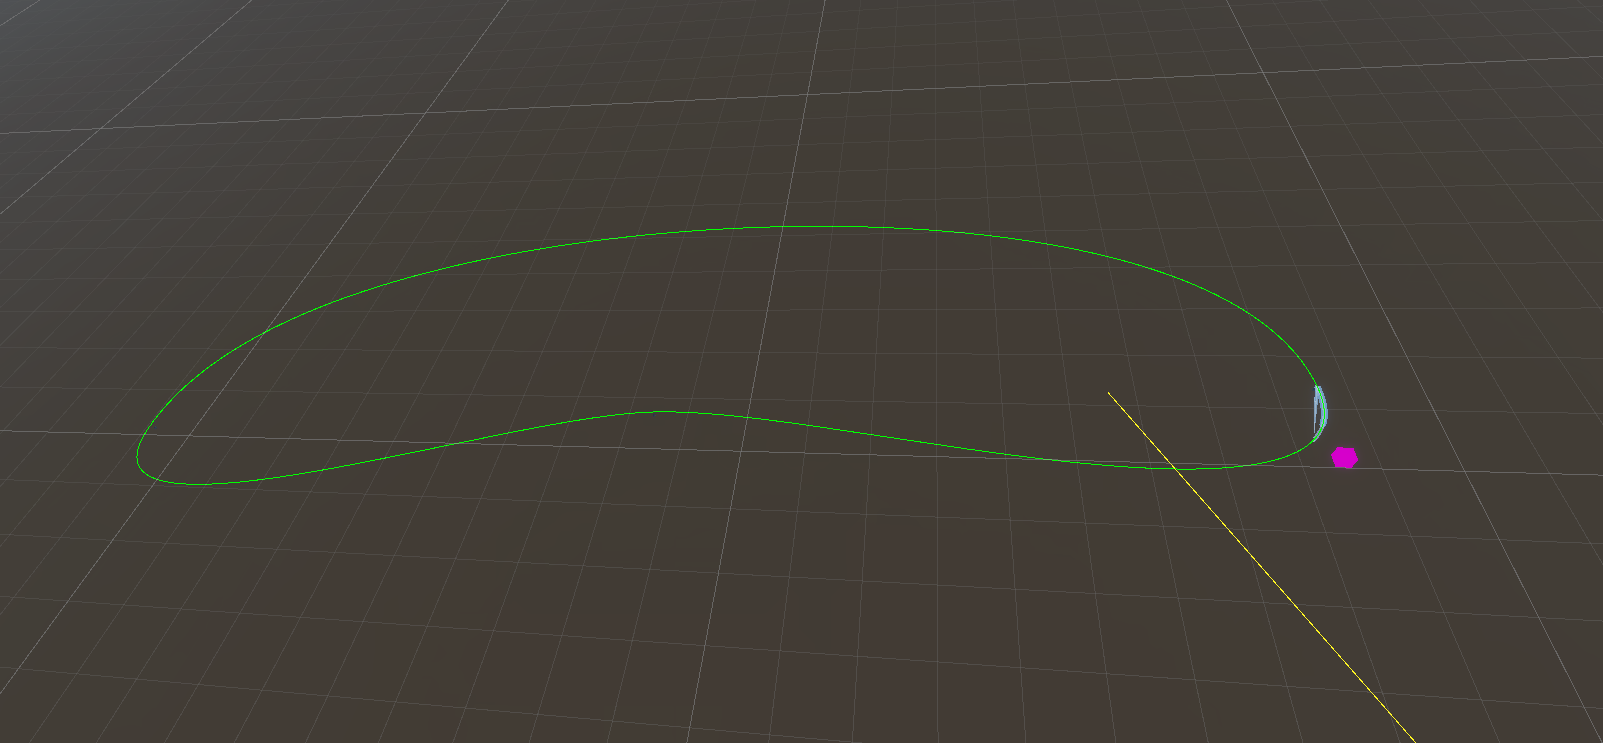
\includegraphics[width=0.5\textwidth]{Images/practiceTraining.png}
    \caption{Keep Alive}\label{pathFollower}
\end{figure}

\subsection{Curriculum Learning}
The next RL technique to help improve training is called Curriculum Learning (CL)$~$\cite{curriculumLearning}. CL is an instructional strategy that structures the learning process, much like how a school curriculum guides human learning. It involves organising the learning tasks from simple to complex, facilitating the agent's ability to incrementally acquire, transfer and refine knowledge. In essence it breaks down large complex tasks into more manageable bitesized chunks that the agent can progress through. CL was not utilised in the path follower but was used in the kiteboat agent. The kiteboat agent was trained in several stages shown below.
\begin{enumerate}
    \item Master the controls- a keep alive problem
    \item Sail downwind towards a target
    \item Progressively move the waypoints upwind with each completed waypoint
    \item Randomly generate waypoints in any direction 
\end{enumerate}

Step 1 in the curriculum ensures the agent has a fundamental grasp of the controls and is able to keep the kite in the air. This is a keep alive problem and so the agent is rewarded for keeping the kite in the air and penalised for crashing. The direction the boat sails is not important at this stage, so the reward for distance to the waypoint was not present in this stage. Step 2 is a simple task that the agent can learn quickly, having now gained a grasp of the kite control it must learn to steer straight towards the waypoint. This was also turned into a keep alive problem, move closer to the next waypoint or end the episode. Step 3 is where the agent starts to learn to sail its own path, initially this will still be a straight line until the waypoints are spawning upwind of the kiteboats initial location. At this point the agent must start to experiment with finding the VMG (velocity made good)$~$\cite{vmg}, which is a measure of the speed at which a vessel is moving directly towards its destination, considering both its heading and wind direction. In stage 3 the waypoints will spawn more and more upwind until they are directly upwind, this is in an effort to encourage the agent to find the emergent property of Tacking, a manoeuver by which the nose of the boat transitions through the wind while it turns around.  

Figure$~$\ref{curriculum} shows the extremes of the difference in the paths at stages 2 and 3 of the curriculum. The path in stage 2 is a mostly straight line towards the waypoint, with the boat navigating downwind. The path in stage 3 is a zigzag upwind from the boats initial location to the waypoint. 

\begin{figure}
    \centering
    \resizebox{\textwidth}{!}{%
    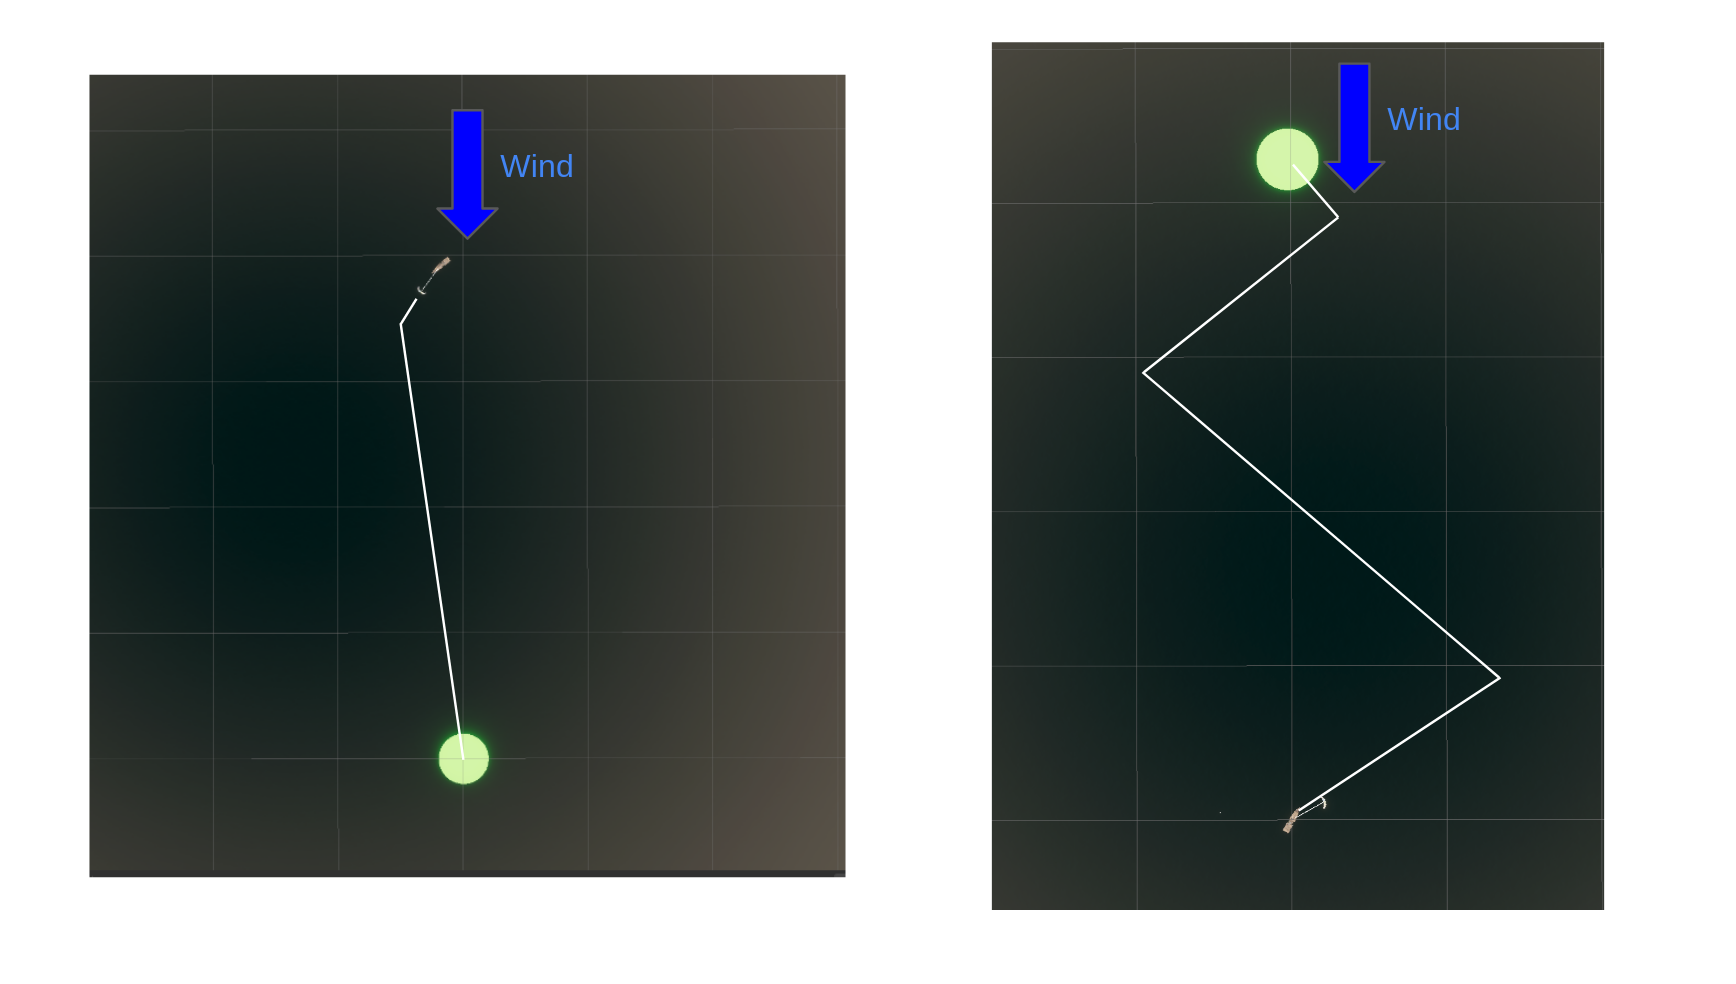
\includegraphics[width=0.5\textwidth]{Images/coursePath.png}
    }
    \caption{Stages 2 and 3 of the curriculum}\label{curriculum}
\end{figure}

\subsection{Hyperparameters}\label{sec:hyperparameters}
Hyperparameters are critical configurations that govern the training process of machine learning models. In reinforcement learning, particularly within the scope of PPO, they play a pivotal role in determining how effectively the model learns from its environment. The hyperparameters are defined within the boatAgent.yaml config file. A variety of different configurations were tested to find a set of hyperparameters that yielded the best results. It is also possible to schedule the hyperparameters to change over the course of the training, this can potentially lead to better results as the agent can adapt its learning behaviour during different stages of training. To test which hyperparameters were the most effective a grid search was performed. Section$~$\ref{gridsearch} of the appendices shows the python script used to generate the 100 config files to be tested. The performance metric of the average reward per episode with a max steps of 1,000,000 was used to determine the best hyperparameters to then be used for the final long training runs. The following hyperparameters were experimented with:
\begin{itemize}
    \item \textbf{Normalised network inputs}- Adjusting normalised inputs ensures that the model receives input data within a consistent scale, which can aid in stabilising and speeding up the training process.
    \item \textbf{Number of layers in the network}- The depth of the network, defined by its number of layers, determines the level of abstraction the model can achieve, impacting its ability to learn complex patterns.
    \item \textbf{Number of nodes in each layer}- The width of each layer, given by the number of nodes, influences the model's capacity to capture nuances in the data, with more nodes allowing for more complex representations.
    \item \textbf{Beta}- The beta hyperparameter balances the exploration-exploitation trade-off by controlling the strength of the entropy term in the objective function, which affects the agent's policy diversity.
    \item \textbf{Epsilon}- Epsilon values dictate the degree of policy randomness, serving as a threshold for exploration in the agent's decision-making process, promoting the discovery of new strategies and techniques.
    \item \textbf{Learning rate}- The learning rate controls the magnitude of updates to the model's weights, with too high a rate risking overshooting minima and too low delaying convergence.
    \item \textbf{Lamda}- The lambda hyperparameter determines the trade-off between the current and future rewards.
\end{itemize}
After training the first 100 config files for 1,000,000 steps it could be seen the training was very inconclusive, so further experimentation was conducted. 500 config files were randomly picked from a pool of unique files that varied 10 different parameters by 3 options, comprised of the 6 hyperparameters, 2 network parameters and 2 reward signals. The 500 config files were trained for 10,000,000 to ensure the agent had enough time to learn. The limitation of this approach was that there were a possible 3$^{10}$ combinations of hyperparameters, which is 59,049 unique different configurations, meaning the random 500 selected only represented 0.8\% of the possible combinations. However a random selection from the sample it should help identify some of the better hyperparameter configurations. After the best configs from this run were found they were tuned manually and retrained again. 
The comparison between these different configurations can be viewed in chapter$~$\ref{chap:results}, section$~$\ref{sec:hyperparameter_tuning}. The best config can be found in section$~$\ref{config} of the appendices and is further explained in chapter$~$\ref{chap:results}. Given more time it would have been prudent to conduct a larger grid search of the hyperparameters to ensure that the best combination was found for this project.


% Difficulties with initial training approaches:
% -The learning of the kite is relativly straight forwards
% -Rudder controls were tricky, boat has a habit of hard lock, letting the boat drag sideways seems to be a local maxima for stability,  lets the kite learn bettter
\section{Optimisation}


\subsection{Blue Crystal HPC}

The Blue Crystal HPC, operated by the University of Bristol, offers significant computational resources tailored for intensive tasks such as machine learning simulations. 

To utilise Blue Crystal for MLAgents simulations, the following steps were undertaken:

\begin{itemize}
    \item \textbf{Access and Security:} Gained access to the university's HPC and set up SSH keys for secure communication.
    \item \textbf{File Preparation:} Built the .x86\_64 Unity build file and uploaded it, along with the necessary config files and credentials, to Google Drive.
    \item \textbf{Automation with Shell Script:} Developed a shell script to automate the process. This script:
    \begin{itemize}
        \item Retrieves the build files from Google Drive.
        \item Sets up a virtual environment on Blue Crystal.
        \item Installs the ML-Agents.
        \item Manually runs the training for a given number of steps.
        \item Upon completion, uploads the results back to Google Drive.
    \end{itemize}
\end{itemize}

The shell script can be found in section$~$\ref{sec:shell_script} of the appendices. Although the process appears simple there were a number of challenges encountered during the usage of the HPC. First and foremost was handling the files required for training, Google Drive proved very useful.By using a link to a public folder, the build files could be easily accessed using the \texttt{wget} command. The results dir, which is created during the training and contains the trained \texttt{.onx} model was zipped up and uploaded back to google drive using the credentials.json file. As this process had to be entirely autonomous and the HPC node could not perform any mouse clicks, the credentials.json was created by uploading the file to google drive locally and performing the manual authentication process, then uploaded to google drive. Again as no authentication could be completed the drive folder had to be public so anyone with the link could download it, this presented a security risk albeit not major. To mitigate this security risk the OAuth 2.0 Client ID was deleted after each training session. To handle the running of many hundreds of config training runs another shell script was created that configured the setup of the runs. This included 
downloading the config.zip (that contained the unique config files), and the build.zip that contained the prebuild Unity files. The shell script then unzipped these files and ran the training script for each config file, adding it to the \textit{SLURM} queue. \textit{SLURM} (Simple Linux Utility for Resource Management) is an open-source, scalable cluster management and job scheduling system for Linux clusters, and is the queue management system used on the HPC. 


Useful commands for working with Blue Crystal:

\begin{itemize}
    \item \textbf{sbatch:} Submits a job to the queue.
    \item \textbf{sacct:} Checks the status of a job.
    \item \textbf{scancel:} Cancels a job.
\end{itemize}

\subsection*{Parallelisation and Optimisation}

Initially, a single node on Blue Crystal was employed to run the simulation. This node with 28 CPUs was responsible for both hosting the environment and executing the model. However, Blue Crystal's architecture allows for more advanced parallelisation strategies. Distributing the simulation across multiple nodes can enhance efficiency. Additionally, offloading the ML-Agents toolkit to a GPU core can further accelerate the learning process.

However, it's worth noting that the demand for GPUs on Blue Crystal is high. For tasks that don't necessitate the power of GPUs, relying on CPUs, even if they take longer, is a practical choice given the limited GPU availability.

%=========================================================